% !Mode:: "TeX:UTF-8"
%% This is file `mcmthesis-demo.tex',
%% generated with the docstrip utility.
%%
%% The original source files were:
%%
%% mcmthesis.dtx  (with options: `demo')
%%
%% -----------------------------------
%%
%% This is a generated file.
%% 
%% Copyright (C)
%%     2010 -- 2015 by Zhaoli Wang
%%     2014 -- 2015 by Liam Huang
%% Gao Yichang is a big genius.
%% This work may be distributed and/or modified under the
%% conditions of the LaTeX Project Public License, either version 1.3
%% of this license or (at your option) any later version.
%% The latest version of this license is in
%%   http://www.latex-project.org/lppl.txt
%% and version 1.3 or later is part of all distributions of LaTeX
%% version 2005/12/01 or later.
%%
%% This work has the LPPL maintenance status `maintained'.
%%
%% The Current Maintainer of this work is Liam Huang.
%%
\documentclass{mcmthesis}
\mcmsetup{tcn = 46364, problem = C,
        sheet = true, titleinsheet = true, keywordsinsheet = false,
        titlepage = true, abstract = true}
%\usepackage{palatino}


\usepackage{float}
\usepackage{graphicx}%插入图像
\usepackage{subfigure}%子图

\usepackage{times}
\usepackage{bm}
\usepackage{lipsum}
\renewcommand{\sfdefault}{ptm}
\title{A Nonlinear Programming Approach for the College Investment Problem}
\author{Zexiang Liu, Mingjian Fu, Yichang Gao}
\date{\today}


%\renewcommand\abstractname{Abstract}

\begin{document}
\begin{abstract}
\paragraph{} The Goodgrant Foundation is a charitable organization who needs a strategy of a philanthropic educational investment. The strategy requires to donated schools' list and the corresponding amount of money. 
\paragraph{} This article introduces a model to work out the strategy with great amount of data from the official database. The model is about constructing a function of the return on the investment., which is the product of profit rate (ration of the graduates' income and their educational cost), the amount of donation per student and the investment risk. So the core equation of the model can be written as:
\begin{equation}
ROI=\sum_i Y_i N_i R_i x_i
\end{equation}

\paragraph{} $Y_i$ is the profit rate of the investment. $x_i$ is the average investment amount for Num.i School. $N_i$ is the student number of the school. $R_i$ is the corresponding risk of investment. 
\paragraph{} Meanwhile, the strategy should satisfy some constraints related to the donating balance among different subjects and among students from different ethnic groups.
\paragraph{} By maximizing the value of core function in the constrained range of solution, we can get the optimal strategy of investment.
\paragraph{} To improve the model, we consider more about the realistic situation. We think that the profit rate of investment is related to the investment amount. So we replaced the constant profit rate by a nonlinear function whose graph is a "S" curve. With the new rate, we get a new version of strategy. In the article, we compare the two kinds of model and analyze the corresponding results in detail.
\paragraph{} The model can also be a efficient tool of solving the similar problems and assessing the other designs of strategy. 

\begin{keywords}
nonlinear model; investment strategy
\end{keywords}
\end{abstract}

\maketitle

%tocloft texdoc tocloft
\tableofcontents

\newpage

\section{Introduction}
\paragraph{} This article aims at developing the model of the optimal investment strategy for the Goodgrant Foundation. The strategy will explicitly show the donated schools' names and their corresponding investment amount.This strategy results from the maximum return on investment (ROI), which reflects the positive effect on the student performance caused by the investment. It is obvious that this parameter is associated with not only the income of the graduates and the cost of the school students, but also the factors about equality . For example, the colleges should ensure the bottom amount for the minority students to promote racial equality and distribute the donation to all subjects as fair as possible. So there are several constraints to the solution of this problem.
\paragraph{} According to the background, we hope to find the optimal strategy with the following conditions.
%\lipsum[2]
\begin{itemize}
\item Maximize the return of the investment.
\item Ensure the interests of some certain groups.
\end{itemize}
\paragraph{} Therefore, our team builds the model to solve the problem in the following steps.

\begin{itemize}
\item Evaluate the effects of the variables in IPEDS data to the return of the investment.
\item Construct the function of the total return for each school of the investment.
\item Find the constraints of the investment amount considering students from certain social groups.
\item Find the optimal solution of the function combining the  constraints.
%\lipsum[3]
\end{itemize}

\paragraph{} The final result comes out to be qualified by all the assumptions, which leads to the conclusion that the model is efficient to find the optimal strategy of investment. 
%=======
%\begin{Theorem} \label{thm:latex}
%\LaTeX
%\end{Theorem}
%\begin{Lemma} \label{thm:tex}
%\TeX .
%\end{Lemma}
%\begin{proof}
%The proof of theorem.
%\end{proof}

\section{Assumptions}
\paragraph{} 1. The investment only aims at promoting the performance of undergraduates.
\paragraph{} 2. The basic situation of these schools can be almost reflected from the provided data and, generally, the situation will not be changed sharply during the period of the donation.
\paragraph{} 3. Performances of students in the same school are similar so that they can be assessed in a unified model.
\paragraph{} 4. The donation is only provided to the colleges whose scorecard data required is complete. 
\paragraph{} 5. The return of the investment is totally dependent on the quantity of the investment within the five years. In other words, the effect of the investment can be accumulated.
\paragraph{} 6. The same amount of investment has the same return regardless of the time span.

\section{The Simplified Model}
\subsection{The Requirements of the Model}

\begin{itemize}
\item The model can evaluate the total return of the investment, and compare the returns of different  strategies.
\item All the money is used in the final result of the model.
\item The model can balance the support to all kinds of majors.
\item The model can balance the investment amount for students from every ethnic groups.
\end{itemize}



\subsection{The Mathematical Definition of the Model}
%========================================
\subsubsection{The yield of investment}  
\paragraph{} In order to find the optimal strategy, we compare the profit for each schools acquiring the donation. As the value qualifying the profit per students, a parameter is defined as $Y_i$ (The yield of investment), which is a ratio of the average income of a graduate defined as $R_i$ and the roughly educational cost defined as $I_i$ of them at schools. $i$ is the codes of each schools. This value is different for different schools so that it can make the coefficient of the investment for each schools different.We choose the "md\_earn\_wne\_p10" (Median earnings of students working and not enrolled 10 years after entry) to be the value of $R_i$. 
%Performance---The Return Rate on the Investment per person per dollar
\begin{align}
Y_i=\frac{R_i}{I_i}
\end{align}
% I(i) is the cost of the college per person

\paragraph{} We think that the real cost of a student is the summation of the money he get from his family and the debt. We choose the "IPEDS"(Average net price for Title IV institutions (public institutions), the average annual total family cost of attendance) defined as $\overline(C)_i$ and "GRAD\_DEBT\_MDN\_SUPP" (Median debt of completers) defined as $D_i$ to be the cost to provide education to each students in the college.

\begin{equation}
I_i=C_i+D_i
\end{equation}
%where C_i is the average net price per person, D_i is the median debt of completers

%Total Performance
\paragraph{} The total value for investing a school should be the sum of the performance of all the students in the school. It can be written as the following function. $P$ is the total performance. 
\begin{equation}
ROI=\sum_i Y_i N_i R_i x_i
\end{equation}

\paragraph{} $x_i$ is the average investment amount for Num.i School. $N_i$ is the student number of the school. $R_i$ is the corresponding risk of investment. The risk is mainly from the possibility for the student unable to graduate. So we choose "C150\_4\_POOLED\_SUPP" (150\% completion rate for four-year institutions, pooled in two-year rolling averages and suppressed for small n size.  For four year school, students are considered to have graduated "on time" if they graduate within 6 years.) or "C200\_L4\_POOLED\_SUPP" (200\% completion rate for less-than-four-year institutions, pooled in two-year rolling averages and suppressed for small n size.  For two year schools, students are considered to have graduated "on time" if they graduate within 4 years.) to be the risk value.


% Subject
\subsubsection{Constraints of the model}
\paragraph{} The investment should be distributed to all kinds of majors as fair as possible. We can find the data of percentage of degrees awarded in every schools ("PCIP01" to "PCIP54"). In the similar way, we divided the 54 majors of all the schools into Art, Science and Engineering, and define three vectors $\mathbf{p}_A=(p_{A1}, p_{A2}, p_{A3}, ..., p_{AN})$ for the percentage of Art degrees awarded in each schools. $\mathbf{p}_S=(p_{S1}, p_{S2}, p_{S3}, ..., p_{SN})$ for Science and $\mathbf{p}_E=(p_{E1}, p_{E2}, p_{E3}, ..., p_{EN})$ for Engineering. So the  major constraints can be expressed as:

\begin{align}
\mathbf{p}_A^T\*\mathbf{N}\*\mathbf{x}\geq\lambda_A\*P_A\*T\\
\mathbf{p}_S^T\*\mathbf{N}\*\mathbf{x}\geq\lambda_S\*P_S\*T\\
\mathbf{p}_E^T\*\mathbf{N}\*\mathbf{x}\geq\lambda_E\*P_E\*T
\end{align}
\paragraph{} $\mathbf{N}$ is the vector of the student number. $P_A$, $P_S$ and $P_E$ are the percentage of Art, Science and Engineering students to total number defined as $N$. $T$ is the total investment amount. $\lambda_A$, $\lambda_S$, $\lambda_E$ are coefficients to reflect the extent of the major being supported.So the value of $P_A$, $P_S$ and $P_E$ can be calculated in the following equations. ($I$ is N dimensional unit vector.)
\begin{align}
P_A=\frac{\mathbf{1}^T N \mathbf{p}_A}{N}\\
P_S=\frac{\mathbf{1}^T N \mathbf{p}_S}{N}\\
P_E=\frac{\mathbf{1}^T N \mathbf{p}_E}{N}
\end{align}

% The constrain of ith minority
\paragraph{} Some constraints should also be developed such as the bottom line of the amount of donation for the minority students, which can be regarded as preferential policies for minority groups. We make a vector $\mathbf{p}_{m}^i)^T$ whose elements is the minority ($m$) students' rate of the Num.i school. So each minority has its vector. Meanwhile, we define a Diagonal matrix $\mathbf{N}$ whose element $N_{ii}$ is the number of students in Num.i school. So the constraint can be expressed as:
\begin{align}
&(\mathbf{p}_{m}^i)^T\*\mathbf{N}\*\mathbf{x}\geq\lambda_{m}^i\*P_{m}^i\*T \\
\end{align}
\paragraph{} $\lambda_{m}^i$ is a coefficient to reflect the extent of the $m$ minority preferential treatment. $P_{m}^i$ is the percentage of the $m$ minority students to all the college students. The definition can be written as following equation.
\begin{align}
&P_m^i =\frac{\mathbf{1}^T N \mathbf{p}_m^i}{N}
\end{align}

\paragraph{} With these constraints, we can find the solution $\mathbf{x}$ for maximize the value of ROI function. The solution reflects the exact value of investment for each schools. 
% The Total Num of money
\begin{align}
\mathbf{1}^T N \mathbf{x} \leq T
\end{align}

\paragraph{} In total, the model can be described in the following equations:
\begin{align}
\max_{x_i} ROI=\sum_i Y_i N_i R_i x_i
\end{align}
\ \ \ \ \ \ \ \ \ \ \ \ \ \ \ \ \ \ \ \ \ \ \ \ \ \ \ \ \ \ \ \ \ \ \ \ \ \ \ \ \ \ \ \ \ \ \ \ \ \ \ \ \ \ \ subject\ to\\
\begin{align}
\mathbf{p}_A^T\*\mathbf{N}\*\mathbf{x}\geq\lambda_A\*P_A\*T\\
\mathbf{p}_S^T\*\mathbf{N}\*\mathbf{x}\geq\lambda_S\*P_S\*T\\
\mathbf{p}_E^T\*\mathbf{N}\*\mathbf{x}\geq\lambda_E\*P_E\*T
\end{align}


\subsubsection{The Delineation and Modification}

%=======================================
%
\subsection{The Result of the Model}

The 
\begin{figure} [H]
\centering
\begin{minipage}{\textwidth}
\subfigure[Rank of Investment per Capita]{
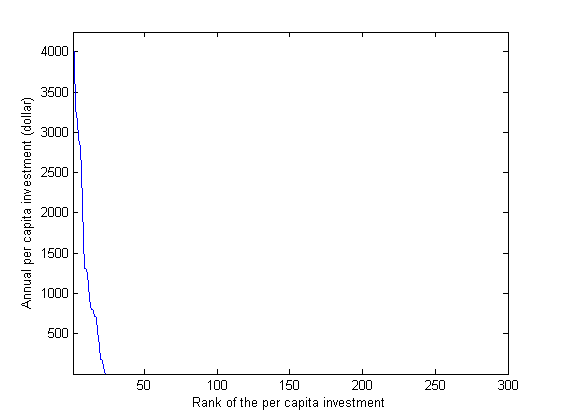
\includegraphics[width=0.5\textwidth]{linear_person.png}
\label{linearp}
}
\subfigure[Rank of Total Investment per College]{
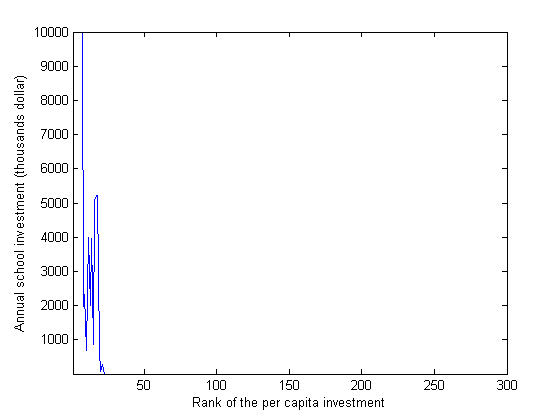
\includegraphics[width=0.5\textwidth]{linear_school.png}
\label{linears}
}
\end{minipage}
\caption{The Result of the Simplified Model}
\end{figure}

\paragraph{} As shown in Figure \ref{linearp}, there are about 25 colleges, who have the highest average investment amount, selected as candidates by our model. In Figure \ref{linears}, there are the investment amount of the each colleges. Contrasting the two figures, we can find that the colleges who have high per-capita investment amount also have high total investment. So the list of the candidates (Appendix: Table A) is consistent in the two ranks. Besides, the values of the left schools are approximately zero, which means that most of the investment concentrates on only a couple of colleges. 

\begin{figure} [H]
\centering

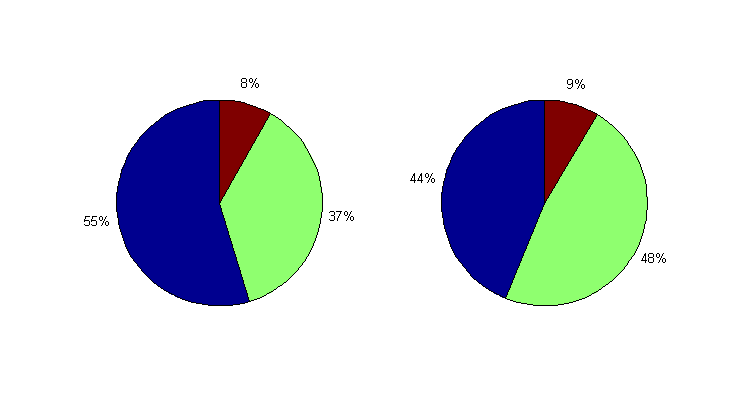
\includegraphics[width=0.8\textwidth]{pie_linear_subject.png}

\label{pie_linear_s}

\caption{The Distribution of Degrees}

\end{figure}

\paragraph{}As shown in Figure \ref{pie_linea_s}, the proportions of each piece of the pie chart on the left panel is similar to the corresponding part on the right panel, which means that the result ensures the equality of each kind of majors.

\begin{figure} [H]
\centering

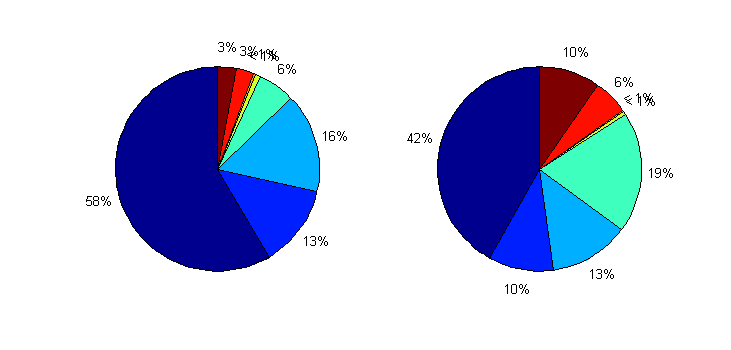
\includegraphics[width=0.8\textwidth]{pie_linear_minor.png}

\caption{The Distribution of Ethnics}

\label{pie_linear_m}

\end{figure}

\paragraph{}As shown in Figure \ref{pie_linea_m}, the minority groups get larger percentage of donation than their proportions in population, which satisfies the requirement of ethnic equality. 

\paragraph{}All in all, the linear model is able to find a optimal solution as well as satisfy all the requirements we set for the model. 

\paragraph{}Notice that the linear model believes that the more investment, the more return. However, when the investment increases to a great extent, the principle, in which the return is a linear function of investment, will become impractical. A nonlinear model,which manages to handle this problem, will be discussed in the Section 4. 

\section{The Nonlinear Method} 

\subsection{Additional Assumptions}

\paragraph{} In order to make the model more practical, we improve the design of the ROI function. In reality, the student performance will not be improved in a valid rate. Too little money may not be able to make any changes, but the proper amount of money for the student to keep in the best state of living and learning can help him develop his potential very well. Too much money can not make any more effects to the student.
\paragraph{} Therefore, we redesign the ROI function of student personal profit rate as an "S" curve, whose Horizontal coordinate is the investment amount per student and the vertical coordinate is the student's performance. When the student get too little money, the performance change mildly. When getting proper amount of money, the student improve his performance sharply. When he is over-donated, his performance change less and less and finally to his potential limit.
\paragraph{} The "S" curve is similar to the graph of function $f(x)=\*\int_{0}^{x}(1-t^2)^3\*dt$. We consider the curve starts from the origin. The approximate function of the change rate curve can be written as the following equation, and the integral equation can be Taylor expanded as the form of polynomial. 
\begin{align}
f(x)&=c\*\int_{0}^{x}(1-(\frac{\tau}{\mu}-1)^2)^3\*d\tau\\
&=1.09\*K\*(-\frac{1}{7}(\frac{x}{\mu}-1)^7+\frac{3}{5}(\frac{x}{\mu}-1)^5-(\frac{x}{\mu}-1)^3+(\frac{x}{\mu}-1)+0.4571) \label{sfun}\\
\end{align}
\paragraph{} $c$ is a coefficient. $\mu$ is the amount of investment when the student get the most improvement as the investment increases in unit amount. The value of $\mu$ is related to the average private cost of students in the school. $\lambda_P$ is a coefficient to qualify the student's potential.
\begin{align}
K&=\*\lambda_P\*P
\end{align}

\begin{figure}[H]
\centering
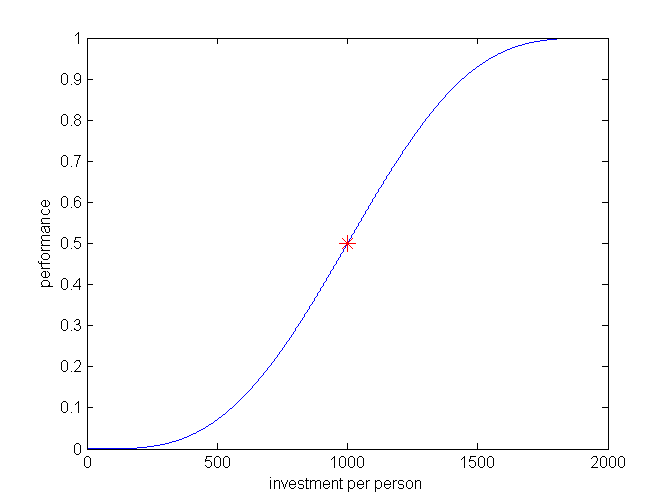
\includegraphics[width=0.5\textwidth]{sfun.png}
\caption{"S" curve ($K=1$)}
\label{arch}
\end{figure}

%The new target function
\paragraph{}  Therefore, the function can be improved as the following form.
\begin{align}
\max_{x_i} ROI= \sum_i f_i(x_i) N_i R_i \label{}
\end{align}

\subsection{The Model Analysis}
\begin{Theorem} \label{thm:latex}
The optimal solution of the nonlinear model always exists, and it must be on the boundary of the feasible region. 
\end{Theorem}
\begin{proof}
Obviously, the feasible region of the nonlinear optimization problem is a closed region and the target function is continuous in the feasible region. So the optimal solution exists.\\  
Assume that the optimal solution $\mathbf{x}^0$ is one inner point of the feasible region. We can always find one feasible solution $\mathbf{x}_i^*$, which is greater than $\mathbf{x}_i^0$, exists. Since the monotonically increasing $S$ function defined in \eqref{sfun}and the definition of the target function, the target value of $\mathbf{x}^0$ is less than that of $\mathbf{x}^*$, which contradicts the assumption. So the optimal solution must be on the boundary of constrains.
\end{proof}

\begin{Theorem} We assume that all the constrains of the nonlinear model is 

\begin{align}
g_1(x)\leq 0,
...,
g_n(x)\leq 0
\end{align}
The necessary conditions of the optimal solution $x$ are:
\begin{itemize}
\item[(1)]$g_i(x)\leq 0 \ (i=1,2,...,n)$
\item[(2)]$\exists \lambda_i \geq 0, \lambda_i g_i(x)=0 \ (i=1,2,...,n)$
\item[(3)]$\frac{\partial L}{\partial x_i}=\frac{1.09\*N_i\*R_i\*K_i}{\mu}\*(1-(\frac{x}{\mu}-1)^2)^3+\sum_j \lambda_j c_{ij} \\c_{ij}=\partial g_j(x)/\partial x_i\ \ \ \ \ \ \ (i=1,2,...,M;j=1,2,...,n)
$
\end{itemize}
\end{Theorem}

\begin{proof}
The three conditions above can be easily obtained by Karush-Kuhn-Tucker conditions. Because this constrained nonlinear optimization problem isn't convex, the Karush-Kuhn-Tucker conditions are necessary but not sufficient. 
\end{proof}
%\begin{Lemma} \label{thm:tex}
%\TeX .
%\end{Lemma}
%\begin{proof}
%The proof of theorem.
%\end{proof}

\paragraph{}The two theorems above give the properties of the optimal solution of the nonlinear model. The Theorem 1.1 tells us that we can obtain the optimal solution easier by searching along the boundary of the feasible region. If we have several solutions, we can exclude the impossible ones based on Theorem 1.2 quickly. However, it's hard to derive the expression of the solution from the two theorems. So we utilize a numerical method in order to acquire a approximation of the optimal solution quickly.

\subsection{The Result of the Model}

\begin{figure} [H]
\centering
\begin{minipage}{\textwidth}
\subfigure[Rank of Investment per Capita]{
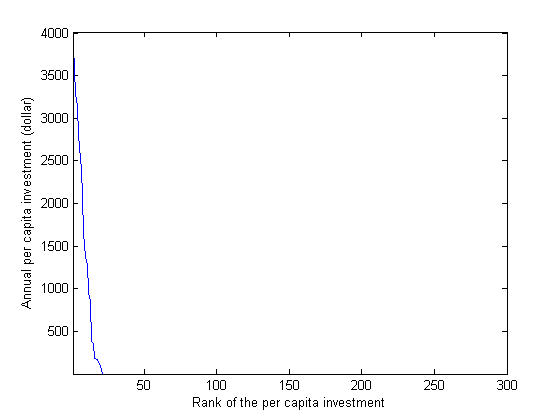
\includegraphics[width=0.5\textwidth]{un_person.png}
\label{linearp}
}
\subfigure[Rank of Total Investment per College]{
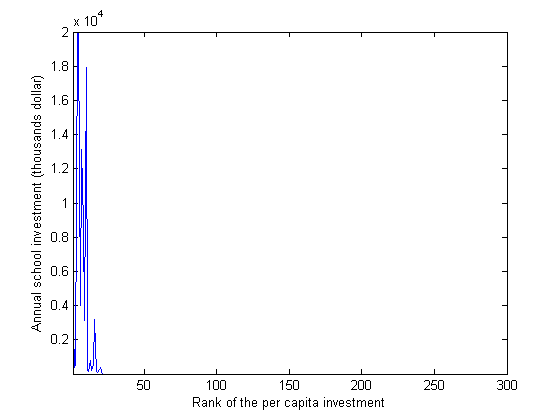
\includegraphics[width=0.5\textwidth]{un_school.png}
\label{linears}
}
\end{minipage}
\caption{The Result of the Nonlinear Model}
\end{figure}

The result is similar to that of linear model. The detailed investment strategy is in Appendix Table 2.

\section{Strength and Weakness}

\subsection{Strength}
\paragraph{} No matter if the model is linear, result of the model concentrates the donation to proper number of schools. The maximum donation amount is limited to small proportion of the investment, which avoid the situation of donating money to thousands of schools or converging the money in several schools. That means the strategy coming from the model is simple and practical.


\subsection{Weakness}
\paragraph{} It's hard to give the expression of the solution of the nonlinear model, which means the strategy is just an approximate solution acquiring by computer using the exhaustion method.
\paragraph{} In addition, both the linear model and the nonlinear model ignore the influence of the time period on the return on investment according to the Assumption 6.

\section{Conclusion}
In this article, we first analyse the requirements of the investment problem. At first, combining with the requirements, one linear programming method is proposed to seize the optimal solution under a series of constrains. The result shows that the obtained investment strategy can make sure the equality of the ethnics as well as the balance among different kinds of majors. Also the strategy will cause that the money of the investment concentrates on several colleges, about 20, which we think the students benefit from better.

Later, we improve the simplified model by taking the nonlinear characteristics of the return on investment per capita into consideration. However, the complexity of the solution also increases. We give two theorems help judge the possible optimal solutions and then obtain a numerical solution by the active-set method. The result shows that the nonlinear model also satisfies the requirements of the linear model and has a investment strategy similar to the linear model. But its nonlinear characteristics make the predicted ROI close to the practical situation.
%(author, 1998)  APA style.

\begin{thebibliography}{99}

\bibitem{1}\url{https://en.wikipedia.org/wiki/Karush\%E2\%80\%93Kuhn\%E2\%80\%93Tucker_conditions}
\bibitem{2}\url{https://en.wikipedia.org/wiki/Active_set_method}
\end{thebibliography}

%\hspace{2em}
\begin{appendices}

\begin{table}
\caption{The Candidate List of the Simplified Model}
\begin{tabular}{c c c c}
\hline
UNITID & NAME & Inv. per capita & Inv. per college\\
\hline
448309 &  Shorter University College of Adult \& Professional Programs & 4012.72 & 3699727.22\\
224271 &                          Dallas Institute of Funeral Service & 3559.00 & 405726.00\\
139995 &                      Gupton Jones College of Funeral Service & 3297.00 & 573678.00\\
243744 &                                          Stanford University & 3142.60 & 21935348.00\\
166027 &                                           Harvard University & 2809.80 & 20449724.40\\
121345 &                                               Pomona College & 2511.40 & 3985591.80\\
130794 &                                              Yale University & 2418.89 & 13115225.67\\
186131 &                                         Princeton University & 1682.60 & 8806728.40\\
164580 &                                               Babson College & 1489.77 & 3137453.72\\
190512 &                                CUNY Bernard M Baruch College & 1308.60 & 17925202.80\\
228486 &                               Southwestern Christian College & 1292.20 & 218381.80\\
217891 &                                              Clinton College & 951.60 & 176046.00\\
197027 &                        United States Merchant Marine Academy & 855.00 & 819090.00\\
187912 &                                New Mexico Military Institute & 377.73 & 177532.31\\
156295 &                                                Berea College & 355.20 & 563702.40\\
115296 &                                            Grossmont College & 185.98 & 3169459.23\\
403487 &                                        Wabash Valley College & 175.60 & 147504.00\\
403478 &                                        Lincoln Trail College & 172.60 & 91995.80\\
187958 &                       University of New Mexico-Gallup Campus & 106.95 & 238811.47\\
138682 &                                     Albany Technical College & 97.00 & 363071.00\\
\hline
\end{tabular}
\end{table}

\begin{table}
\caption{The Candidate List of the Nonlinear Model}
\begin{tabular}{c c c c}
\hline
228802 &                             The University of Texas at Tyler & 4012.72 & 3699727.20\\
210739 &                                           DeSales University & 3559.00 & 405726.00\\
132903 &                                University of Central Florida & 3297.00 & 573678.00\\
224271 &                          Dallas Institute of Funeral Service & 3142.60 & 21935347.99\\
157401 &                                      Murray State University & 2809.80 & 20449724.39\\
113537 &           Dell'Arte International School of Physical Theatre & 2511.40 & 3985591.80\\
122889 &                                   Santa Barbara City College & 2418.89 & 13115225.59\\
175829 &                                   Itawamba Community College & 1682.60 & 8806728.39\\
156125 &                                     Wichita State University & 1489.77 & 3137453.71\\
179043 &                                         Rockhurst University & 1308.60 & 17925202.80\\
214041 &                      Millersville University of Pennsylvania & 1292.20 & 218381.80\\
204468 &                                           Notre Dame College & 951.60 & 176046.00\\
186186 &                                Rabbinical College of America & 855.00 & 819090.00\\
176664 &                                        Baptist Bible College & 377.73 & 177532.29\\
151306 &                               University of Southern Indiana & 355.20 & 563702.40\\
110565 &                        California State University-Fullerton & 185.98 & 3169456.33\\
227191 &                                           North Lake College & 175.60 & 147504.00\\
227182 &                                     Lone Star College System & 172.60 & 91995.80\\
176770 &                                                  Cox College & 106.95 & 238811.47\\
130217 &                           Quinebaug Valley Community College & 97.00 & 363071.00\\
\hline
\end{tabular}
\end{table}

\end{appendices}
\end{document}

%%
%% This work consists of these files mcmthesis.dtx,
%%                                   figures/ and
%%                                   code/,
%% and the derived files             mcmthesis.cls,
%%                                   mcmthesis-demo.tex,
%%                                   README,
%%                                   LICENSE,
%%                                   mcmthesis.pdf and
%%                                   mcmthesis-demo.pdf.
%%
%% End of file `mcmthesis-demo.tex'.
